\begin{figure}[htbp]
\centering
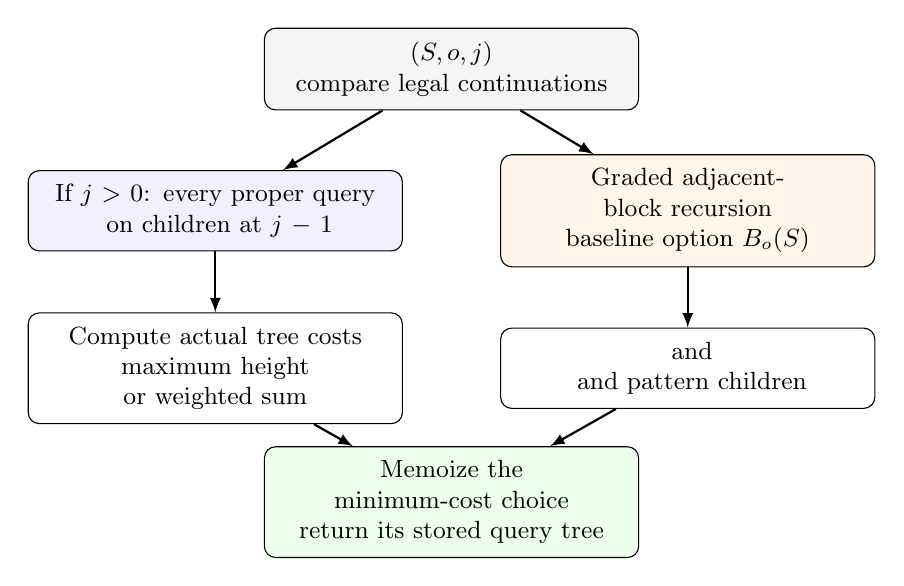
\begin{tikzpicture}[every node/.style={font=\small},
  box/.style={draw,rounded corners,align=center,inner sep=5pt,text width=4.4cm},
  arr/.style={-latex,thick}]
  \node[box,fill=gray!8] (rollout) at (0,0)
    {\Rollout$(S,o,j)$\\compare legal continuations};
  \node[box,fill=blue!6] (split) at (-3,-1.8)
    {If $j>0$: every proper query\\\Rollout\ on children at $j-1$};
  \node[box,fill=orange!8] (baseline) at (3,-1.8)
    {Graded adjacent-block recursion\\baseline option $B_o(S)$};
  \node[box] (grade) at (3,-3.8)
    {\HullData\ and \GradeDP\\\EndpointCode\ and pattern children};
  \node[box] (evaluate) at (-3,-3.8)
    {Compute actual tree costs\\maximum height or weighted sum};
  \node[box,fill=green!7] (best) at (0,-5.5)
    {Memoize the minimum-cost choice\\return its stored query tree};
  \draw[arr] (rollout) -- (split);
  \draw[arr] (rollout) -- (baseline);
  \draw[arr] (baseline) -- (grade);
  \draw[arr] (split) -- (evaluate);
  \draw[arr] (grade) -- (best);
  \draw[arr] (evaluate) -- (best);
\end{tikzpicture}
\caption{Exact lookahead wrapped around the quasipolynomial baseline.
The arrows denote calls and the returned trees or costs. The baseline
completes any branch that reaches its stopping depth. Thus the
logarithmic cap on $j$ bounds the number of search transcripts while
each returned tree still completes identification. The proof compares
this finite search with an optimal tree; the algorithm evaluates only
trees it has constructed.}
\label{fig:qp-procedure-flow}
\end{figure}
